%% ------------------------------------------------------------------------- %%
\chapter{Experimentos Preliminares}
\label{cap:experimentos}

Texto texto texto texto texto texto texto texto texto texto texto texto texto.

%------------------------------------------------------
\section{Conjuntos de dados} 

Para os experimentos foram utilizadas duas bases de dados distintas. A primeira delas, denominada UCI neste trabalho, foi proposta por \citet{uci-skin-dataset:12} e obtida no repositório de aprendizagem de máquina da Universidade da Califórnia em Irvine \citep{lichman:13}. A base é constituída por imagens de várias texturas de pele e não pele obtidas a partir de milhares de imagens arbitrárias de faces de diferentes idades, sexo e raças \citep{pal-texas:04, feret:96}.

A UCI contém 245.057 amostras, compostas por 3 atributos que constituem o vetor de entradas $x = [x_1, x_2, x_3]$, $x \in \mathbb{R}^{d}$, sendo $d$ a dimensão do espaço, e que representam, respectivamente, os canais B (\textit{Blue}), G (\textit{Green}) e R (\textit{Red}) do modelo de cores RGB, além de uma quarta coluna que determina a classe a qual a amostra $x$ pertence, denotada por $y$, sendo $y \in Y$ e $Y = \{+1, -1\}$.

Em outras palavras, cada amostra é um pixel RGB com um determinado rótulo. Como tem-se os dados rotulados com exemplos de qual é a saída correta para uma dada entrada, os experimentos subsequentes são categorizados como sendo de aprendizado supervisionado \citep{mostafa:12}.

A tabela~\ref{tbl:uci_dataset} exemplifica um pequeno trecho da base de dados UCI. Vale ressaltar que do total das 245.057 amostras, 194.198 são de pixels não pele e 50.859 de pixels com diferentes tons de pele. Além disso, as imagens que foram utilizadas na extração do conjunto de dados não foi disponibilizada pelos autores.

\begin{table}[!htpb]
\centering
\begin{small}
\begin{tabular}{|c|c|c|c|} \hline
B       & G     & R     & Classe  \\ \hline
74	    & 85    & 123	& 1     \\
207	    & 215   & 255   & 1     \\
74      & 82    & 122	& 1     \\
202     & 211   & 255   & 1     \\
54      & 72    & 125   & 1     \\
\ldots  &\ldots & \dots &\ldots \\
166     & 164   & 116   & -1    \\
148     & 150   & 91    & -1    \\
29      & 26    & 5     & -1    \\
167     & 166	& 115	& -1    \\
180	    & 177	& 133	& -1    \\ \hline
\end{tabular}
\caption[Trecho com amostras da base de dados UCI]{Trecho com amostras da base de dados UCI. Cada uma das três primeiras colunas representam um canal do pixel do espaço de cores RGB e variam entre 0 e 255. A quarta coluna é a classe atribuída à amostra, que pode assumir +1 se for pele e -1, caso contrário. Originalmente, a classe que representa um pixel de não pele tinha valor 2, substituída por -1 para conformidade com os experimentos.}
\label{tbl:uci_dataset}
\end{small}
\end{table}

Uma vez que a dimensão do espaço do problema é $d = 3$, é possível plotar os dados para melhor interpretação dos mesmos, conforme mostra a figura~\ref{fig:dataset_uci}.
\begin{figure}[h]
    \centering
    \begin{minipage}{0.45\textwidth}
        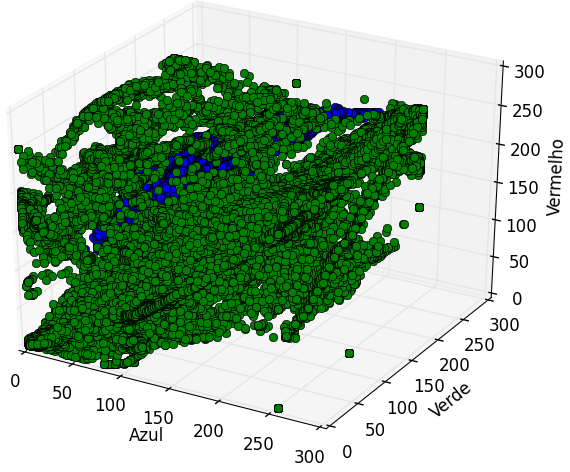
\includegraphics[width=\textwidth]{uci_skinns_plot}
    \end{minipage}
    ~ % space
    \begin{minipage}{0.45\textwidth}
        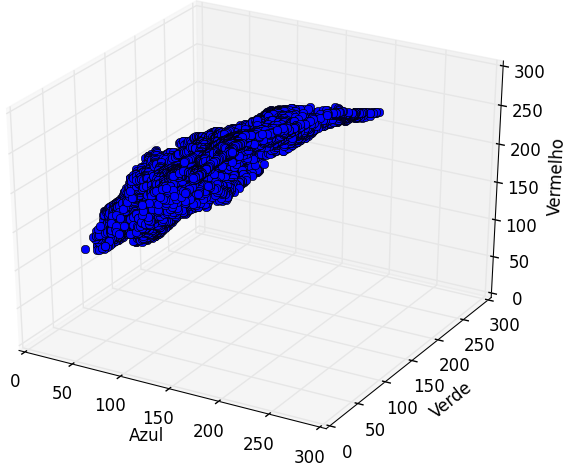
\includegraphics[width=\textwidth]{uci_skin_plot}
    \end{minipage}
    \caption[Visão 3-dimensional dos canais RGB do conjunto de dados UCI]{Visão 3-dimensional dos canais RGB do conjunto de dados UCI. Os pontos em azul são amostras de pele e os verdes de não pele. À esquerda tem-se todas as amostras do conjunto de dados; à direita apenas as amostras de pele. Fonte: proposto pelo autor.}
    \label{fig:dataset_uci}
\end{figure}

O segundo conjunto de dado utilizado nos experimentos foi proposto por \citet{sfa-skin-dataset:13}, intitulado pelos autores como banco de imagens de pele humana baseado no FERET e AR (SFA), cuja sigla também será utilizada neste trabalho. O SFA possui um conjunto de imagens de faces obtidas a partir de outros dois bancos de imagens coloridas: o FERET, criado por \citet{feret:96} e o AR, proposto por \citet{ar-face-database:98}, tendo sido utilizadas 876 e 242 imagens de cada um, respectivamente. É importante ressaltar que as imagens do AR têm fundo branco e pequenas variações de cor da pele e, portanto, o ambiente é mais controlado que as imagens do FERET \citep{sfa-skin-dataset:13}. A figura~\ref{fig:sfa_dataset_exemplo} mostra um exemplo das 1.118 imagens do banco.

\begin{figure}[h]
    \centering
    \begin{minipage}{0.3\textwidth}
        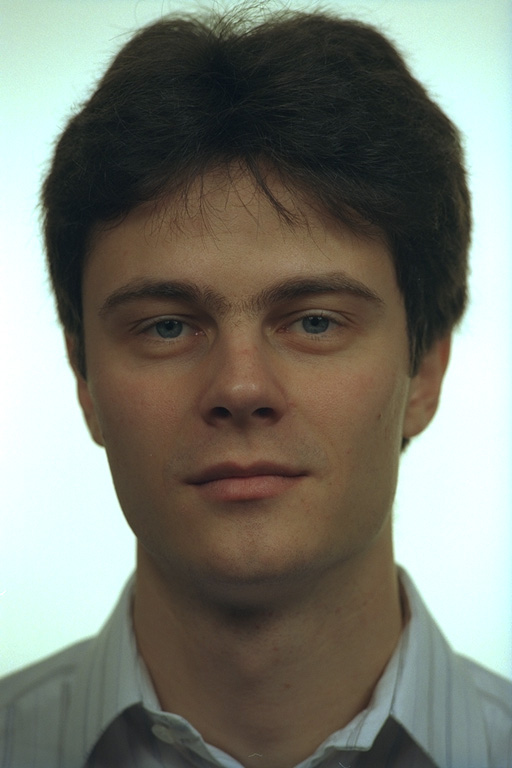
\includegraphics[width=\textwidth]{sfa_img_1}
    \end{minipage}
    ~ % space
    \begin{minipage}{0.3\textwidth}
        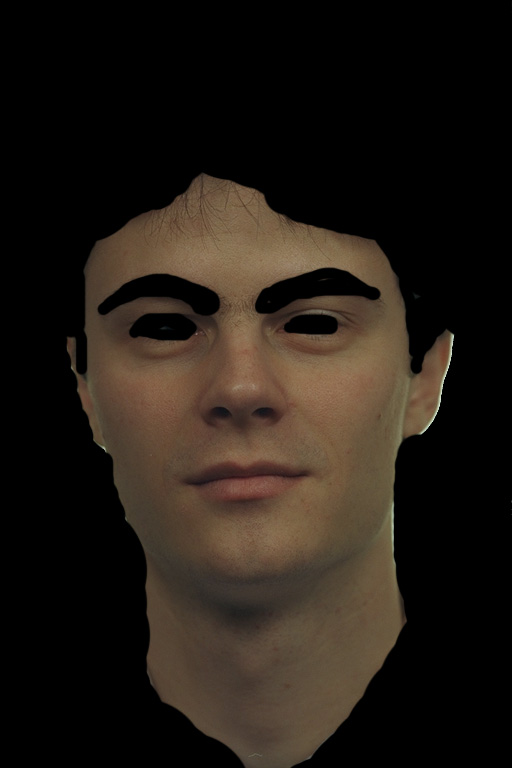
\includegraphics[width=\textwidth]{sfa_img_1_gt}
    \end{minipage}
    \caption[Exemplos de imagens do banco de faces SFA]{Exemplos de imagens do banco de faces SFA. À esquerda a imagem original e à direita o ground truth com os pixels de cor de pele anotados manualmente, sendo que a cor preta RGB = (0, 0, 0) foi atribuída a todos os pixels no fundo. Fonte: \citet{sfa-skin-dataset:13}.}
    \label{fig:sfa_dataset_exemplo}
\end{figure}

As amostras de pele e não pele foram geradas aleatoriamente considerando a máscara \emph{ground truth}\footnote{\emph{Ground truth} é o termo utilizado para denotar uma imagem cujo objeto de interesse está devidamente segmentado e ressaltado, descartando os pixels remanescentes atribuindo-lhes cores uniformes.} de cada imagem, sendo três amostras de pele e cinco de não pele. Cada amostra é uma janela de tamanho $n\times n$, sendo $n$ ímpar, com um pixel central, a partir do qual outros tamanhos de amostra foram criados, que variam de $1 \times 1$ até $35 \times 35$, como pode ser visto na figura~\ref{fig:sfa_dataset_janelas} \citep{sfa-skin-dataset:13}.

\begin{figure}[h]
  \centering
  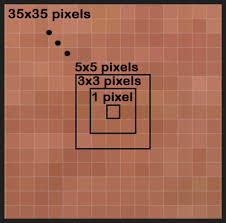
\includegraphics[width=.35\textwidth]{sfa-janelas}
  \caption[Estrutura das janelas que formam as amostras do SFA]{Estrutura das janelas que formam as amostras do SFA. No total, são 3.354 amostras de pele e outras 5.590 de não pele para cada tamanho de janela. Fonte: \citet{sfa-skin-dataset:13}.}
  \label{fig:sfa_dataset_janelas}
\end{figure}

A partir das amostras criadas no SFA, um conjunto de dados foi extraído gerando uma base de dados de pele e não pele similar ao UCI na tabela~\ref{tbl:uci_dataset}. O tamanho da janela utilizado foi $9 \times 9$ e o espaço de cores também foi o RGB. Portanto, o total de amostras empregado nos experimentos é 724.464, sendo 271.674 de pele e 452.790 de não pele. A classe atribuída à cada amostra tem o mesmo valor que no UCI, ou seja, +1 se for pele e -1, caso contrário. A figura~\ref{fig:dataset_sfa} mostra a representação gráfica dos dados plotados em 3 dimensões.
\begin{figure}[h]
    \centering
    \begin{minipage}{0.45\textwidth}
        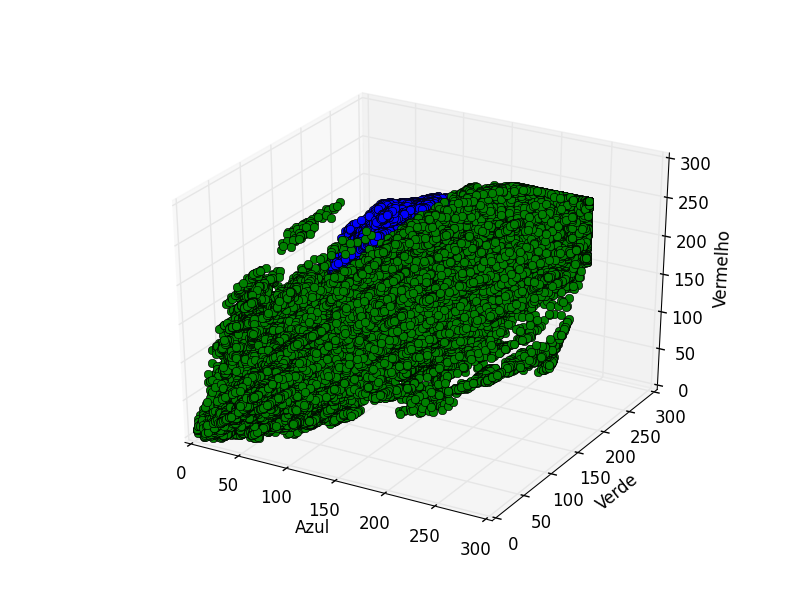
\includegraphics[width=\textwidth]{sfa_skinns_plot}
    \end{minipage}
    ~ % space
    \begin{minipage}{0.45\textwidth}
        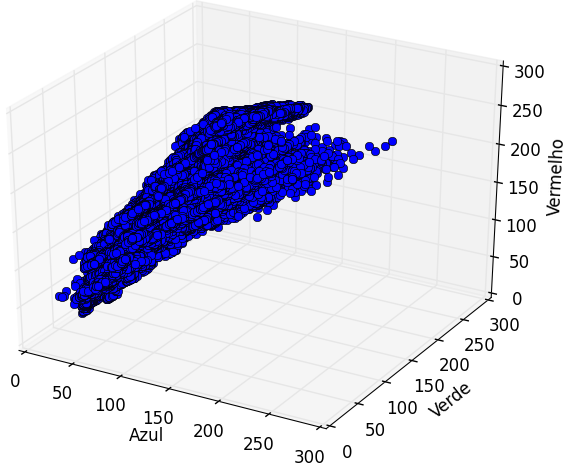
\includegraphics[width=\textwidth]{sfa_skin_plot}
    \end{minipage}
    \caption[Visão 3-dimensional dos canais RGB do conjunto de dados SFA]{Visão 3-dimensional dos canais RGB do conjunto de dados SFA. Os pontos em azul são amostras de pele e os verdes de não pele. À esquerda tem-se todas as amostras do conjunto de dados gerado; à direita apenas as amostras de pele. Fonte: proposto pelo autor.}
    \label{fig:dataset_sfa}
\end{figure}